\documentclass[smallcondensed,final]{svjour3}                     % onecolumn (standard format)
%\documentclass{article}
\RequirePackage{fix-cm}

\usepackage{graphicx}
\usepackage[fleqn]{amsmath}
\usepackage{amssymb}
\usepackage{bm}
%\usepackage{pgf}
%\usepackage[polutonikogreek]{babel}

\begin{document}

\title{Symbolic linearization of equations of motion of constrained multibody systems}

\titlerunning{Symbolic linearization of equations of motion of constrained multibody systems}        % if too long for running head

\author{Dale L. Peterson\and Gilbert Gede\and Mont Hubbard}

\institute{Dale L. Peterson, Gilbert Gede, Mont Hubbard \at
           Sports Biomechanics Laboratory\\
           Department of Mechanical and Aerospace Engineering\\
           University of California Davis\\
           Davis, CA 95616-5294\\
           Tel.: +1 530 752 2163\\
           \email{\{dlpeterson,ggede,mhubbard\}@ucdavis.edu}}

\date{Received: date / Accepted: date}

\maketitle

\begin{abstract}
% Context
Many common mechanical systems have configuration or velocity constraints.
% Need  (what we have and what we want)
Analyses of such systems often require linearized forms of the motion
equations.
% Task
To address this issue, we developed a procedure for organizing the constraint
and motion equations and their subsequent linearization.
This procedure was specifically developed for equations of motion generated by
Kane's method, but is compatible with any method as long as the following are
true: only ordinary differential equations are required to describe the system,
and independent and dependent states remain in the final equations (i.e. no
DAEs, no substitution of variables).
% Object of the document
Following a brief review of Kane's method and the structure of the equations it
generates, we present the procedure to symbolically linearize the nonlinear
motion equations of constrained multibody systems, and illustrate it with the
% TODO: change name of example
familiar example of the rolling disc.


\keywords{linearization, constrained multibody systems, symbolic dynamics, control}
\end{abstract}

%In summary, the procedure is:
%\begin{enumerate}
%    \item Describe the system in the form of the equations shown in Table
%        \ref{table:assumptions}.
%    \item Determine a point of linearization ($\bm{q}^*$, $\dot{\bm{q}}^*$,
%      $\bm{u}^*$, $\dot{\bm{u}}^*$, and $\bm{r}^*$) which satisfies the
%      equations in Table \ref{table:assumptions}.
%    \item Compute the quantities in equation (\ref{eq:quant_to_compute}).
%    \item Identify independent coordinates and speeds; form equations (\ref{eq:C_0}), (\ref{eq:C_1}), and
%        (\ref{eq:C_2}).
%    \item Form equation (\ref{eq:state_space_constrained}), and if needed,
%      equations (\ref{eq:A_prime})-(\ref{eq:B}).
%\end{enumerate}

\section{Introduction}
\label{sec:intro}
Designing a feedback controller or performing stability analysis are two common
analyses performed on models of multibody systems.
A linear form of the equations of motion is required to apply the most
frequently used techniques for the analyses to such systems.
Normally, obtaining the linearized equations of motion is as simple as taking
the Jacobian of the right hand side function of the equations of motion with
respect to the states.
However, when the multibody system in questions has constraints, this process
is more complicated.
If one has used Kane's method \cite{Kane1985} to generate the equations for a
constrained system, the resulting equations will have a particular form: a set
of ordinary differential equations containing both the independent and
dependent states.
Simple inspection of the equations does not reveal that they represent a
constrained system - their form is similar to the equations of an unconstrained
system.
It is critical to understand linearizing these equations by computing the
Jacobian gives incorrect results.
This paper provides a way to correctly generate the linear equations of motion
for constrained systems which have been found using Kane's method (or any other
method which results in equations with the same form).

Multibody systems (rigid or flexible) and particles often have constraints
which limit how they can move or be configured.
In this paper, we will discuss three types of constraints: configuration,
velocity, and acceleration.
Configuration constraints limit the location or orientation of parts of the
system, relative to the external world or other parts of the system.
Velocity constraints limit the speeds at which the configuration can change,
either from configuration constraints (through time differentiation) or
independent application.
Velocity constraints most often appear in systems where there is rolling
without slip or there are closed kinematic loops.
Within this paper, acceleration constraints refer to time differentiated
velocity constraints.

% TODO: Improve literature review.
Bottema appears to be the first author to show that special considerations are
needed for linearizing nonholonomic systems \cite{Bottema1949}.
While other authors have examined linearization of nonholonomic systems, we
have found isssues with applying any of them to equations generated by Kane's
method.
Kang et al. \cite{Kang2003} and Negrut and Ortiz \cite{Negrut2006} have both
explored linearization, but these methods have been developed for equations of
motion found using Lagrange's method, which contain Lagrange multipliers (which
are not present in equations of motion generated from Kane's method).
Minaker and Rieveley \cite{Minaker2010} and Schwab and Meijaard
\cite{Schwab2003} both have developed techniques for generating equations of
motion (and linear forms thereof), however both techniques are more numerical
in nature - they do not provide symbolic equations of motion or symbolic
linearized equations.
These processes, along with others such as Neuman's %TODO: fix reference
, formulate the linear equations as a step in the equations of motion
generation process.
They are not capable of linearizing existing equations of motion.

% TODO:reiterate limiations of model
The goal of this paper is to correctly establish the first order relationships
(about an arbitrary point of linearization) between a selection of independent
coordinates and speeds and the time-derivatives of all coordinates and speeds
(both independent and dependent). The formalism presented here is generic
enough to cover most examples of time-varying constrained multibody systems
with arbitrary external inputs and arbitrary specified quantities.
% TODO: electronic supplementary material with examples for other methods
% TODO: rewrite following sentences after e.s.m.
The
procedure was created for systems whose equations of motion have been derived
with Kane's method. Although also applicable to dynamic system equations
formulated using other methods, it is restricted to systems which can be
completely described by a set of ODEs (i.e., DAEs needn't be solved).

% TODO:rewrite organization of paper
The use of Kane's method in generating equations of motion is reviewed first,
in order to properly orient the reader to the format and some of the qualities
of the generated equations.
Kane's method is then used to generate the equations of motion for a simple
system, 
%TODO: update example name 
a rolling disk with a trailing arm.
The need for a different linearization technique is also demonstrated with this
model.
In response to this need, we present the newly developed linearization
procedure and its derivation.
This new linearization procedure is then performed on the example system to
provide an example of its application.
Finally, we discuss other details and nuances of the procedure and its use.


\section{Kane's Method, Briefly}
\label{sec:kane_method}
To familiarize the reader with Kane's method, some concepts relating to its
use will be described.
The first is the use of generalized speeds in addition to generalized
coordinates.
The second concept is in how these generalized speeds can be used to project
permissible motions of the system, and how this removes the need to consider
non-contributing (internal constraint) forces.
Then, the mathematical steps required to use Kane's method are shown and
described.

When using Lagrange's method, generalized coordinates are used to describe the
configuration of a system while the time derivatives of the gen. coordinates
describe the velocities of a system.
Kane's method allows for the velocities of a system to be written in terms of
generalized speeds, which are not required to be the time derivatives of
coordinates (although such a definition is permitted).

The benefit of using both generalized speeds and coordinates can be seen in
the following example.
If the orientation of a rigid body were to be described using using Euler
parameters (quaternions), its angular velocity is relatively complicated when
using the time derivatives of the coordinates.
Using generalized speeds allows for the angular velocity to be written in the
much simpler form
\begin{align}
\label{eq:ex1}
{^N}\bar{\omega}^B = \it{\omega}_1 \hat{b}_1 + \it{\omega}_2 \hat{b}_2 +
\it{\omega}_3 \hat{b}_3
\end{align}
or, the angular velocity of rigid body $B$ in the reference frame $N$ is the
defined as the sum of three generalized-speed/basis-vector products.
The derivatives of these generalized speeds will then appear in the equations
of motion, rather than the twice time differentiated generalized coordinates
($\ddot{\mathbf{q}}$'s).

A downside of allowing such definitions is clear when formulating the kinematic
differential equations, which relate the rate of change of the generalized
coordinates to the generalized speeds.
These equations become much more complicated, but this is usually offset by the
significantly simpler equations of motion.

Use and understanding of Kane's method requires another concept, partial
velocities.
Partial velocities are defined as the partial derivatives of the velocity
vectors with respect to the generalized speeds.
They are defined for both translational and rotational velocities.
Using the angular velocity of body $B$ in reference frame $N$ as shown in
(\ref{eq:ex1}), the partial velocities can be written
\[
{^N}\bar{\omega}^B_{\omega_1} = \hat{b}_1 \quad \quad
{^N}\bar{\omega}^B_{\omega_2} = \hat{b}_2 \quad \quad
{^N}\bar{\omega}^B_{\omega_3} = \hat{b}_3
\]
and it can be seen that the partial velocities represent the direction of
motion associated with each generalized speed.

By taking the dot product of each partial velocity and both sides of Newton's
second law, $\bar{F}=m\bar{a}$ (or the rotational equivalent), only terms that
are parallel to the partial velocities are left in the equation.
One equation is generated for each generalized speed.

An important byproduct of this is that internal constraint forces
(non-contributing forces) imposed by constructs such as pin or sliding joints
no longer need to be considered.

In summary, Kane's method allows for velocities to be defined in terms of
generalized speeds, allowing for simpler velocity expressions.
The dot product of each partial velocity (the direction of motion associated
with each generalized speed) with Newton's second law (or Euler's equations)
removes all terms which are not related to each generalized speed.
This generally results in simple equations of motion, which are easier to form.

The mathematical formalism for applying Kane's method to multibody systems
follows.
Consider a system composed of rigid bodies $B_1,...,B_g$, particles
$P_1,...,P_h$, with points of force application $Q_1,...,Q_k$, and reference
frames of torque application $E_1,...,E_c$, all defined relative to the
inertial reference frame $N$.
This system has generalized coordinates $q_1,...,q_n$ and generalized speeds
$u_1,...,u_o$.
Additionally, there are $l$ configuration constraints and $m$ velocity
constraints.

In order to properly apply Kane's method, the velocities of each component in
the system need to be written in the following form.

Translational velocity of particles:
\begin{align}
\label{eq:particle_translational}
{^N}\bar{v}^{P_i} = \sum^o_{j=1} {^N}\bar{v}^{P_i}_{u_j} u_j + {^N}\bar{v}^{P_i}_t
\quad \quad i=1,...,g
\end{align}
Translational velocity of rigid body mass centers:
\begin{align}
\label{eq:rb_translational}
{^N}\bar{v}^{B_i^*} = \sum_{j=1}^o {^N}\bar{v}^{B_i^*}_{u_j} u_j +
{^N}\bar{v}^{B_i^*}_t \quad \quad i=1,...,h
\end{align}
Translational velocity of points of interest:
\begin{align}
\label{eq:points_translational}
{^N}\bar{v}^{Q_i} = \sum_{j=1}^o {^N}\bar{v}^{Q_i}_{u_j} u_j + {^N}\bar{v}^{Q_i}_t
\quad \quad i=1,...,k
\end{align}
Rotational velocity of rigid bodies:
\begin{align}
\label{eq:rb_rotational_bodies}
{^N}\bar{\omega}^{B_i} = \sum_{j=1}^o {^N}\bar{\omega}^{B_i}_{u_j} u_j +
{^N}\bar{\omega}^{B_i}_t \quad \quad i=1,...,h
\end{align}
Rotational velocity of reference frames of interest:
\begin{align}
\label{eq:rb_rotational_frames}
{^N}\bar{\omega}^{E_i} = \sum_{j=1}^o {^N}\bar{\omega}^{E_i}_{u_j} u_j +
{^N}\bar{\omega}^{E_i}_t \quad \quad i=1,...,c
\end{align}

In these equations, each term $\bar{v}_t$ or $\bar{\omega}_t$ represents the
velocity or angular velocity component which is a prescribed function of time,
and has no dependence on generalized speeds (e.g., a crank
driven at a fixed rate).

For this system, the configuration constraints are defined as:
\begin{align}
\label{eq:configuration_constraints}
\mathbf{f}_c(\mathbf{q}, t) = \mathbf{0}
\end{align}
where the terms $\mathbf{f}_c$ and $\mathbf{0}$ have the shape $l \times 1$.
The velocity constraints are defined as:
\begin{align}
\label{eq:velocity_constraints}
\mathbf{f}_v(\mathbf{q}, \mathbf{u}, t) = \mathbf{0}
\end{align}
where the terms $\mathbf{f}_v$ and $\mathbf{0}$ have the shape $m \times 1$.
It is important that the velocity constraints include the time-differentiated
configuration constraints or equivalent constraints which produce the same
behavior.
Furthermore, velocity constraints can not be written with $\dot{\mathbf{q}}$
terms (the time derivatives of the coordinates).
Acceleration constraints need to be defined as well.
Typically, they will simply by time-differentiated velocity constraints and
have the form:
\begin{align}
\label{eq:acceleration_constraints}
\mathbf{f}_a(\mathbf{q}, \dot{\mathbf{q}}, \mathbf{u}, \dot{\mathbf{u}}, t) =
\mathbf{0}
\end{align}

At this point, it is convienient to define a matrix $\mathbf{B}$, which is the
gradient of the velocity constraints $\mathbf{f}_v$ with respect to all of the
generalized speeds $\mathbf{u}$.
\begin{align}
\label{eq:constraint_B}
\mathbf{B} \triangleq \nabla_{\mathbf{u}} \mathbf{f}_v (\mathbf{q}, \mathbf{u},
t)
\end{align}
and from (\ref{eq:velocity_constraints}) and (\ref{eq:constraint_B}) the
following can be written:
\begin{align}
\label{eq:constraint_Bu0}
\mathbf{0} = \mathbf{B}\mathbf{u}
\end{align}

With these definitions established, Kane's method can be applied.
The output of Kane's method is the equation
\begin{align}
\label{eq:kanes_eq}
\mathbf{F} + \mathbf{F}^* = \mathbf{0}
\end{align}
or, the sum of the generalized active forces and generalized inertial forces is
0.
If Newton's second law were written as $f - ma = 0$, the $\mathbf{F}$ is the
multibody generalization of $f$ and $\mathbf{F}^*$ is the multibody
generalization of $-ma$.
These terms are created by taking the dot product of the partial
velocities/angular-velocities, as defined in (\ref{eq:particle_translational})
- (\ref{eq:rb_rotational_frames}), with the resultant forces/torques ($\bar{R}$/
$\bar{T}$) and the inertial forces/torques ($\bar{R}^*$/$\bar{T}^*$).

The resultant force at a point is defined as the sum of all force vectors
acting directly on that point.
The resultant torque on a reference frame is defined similarly - it is the sum
of all torque vectors acting on that reference frame.
Note that distance forces do not need to be transformed into a resultant
force/torque pair for any components of the system; they only need to be
considered at the point of application (e.g., if a force $\bar{f}$ is the only
force applied to body $B$ and is applied at point $Q$, then $\bar{R}_{B^*}=0$
and $\bar{T}_B=0$ but $\bar{R}_Q=\bar{f}$).
These resultant forces and torques are used to write the generalized active
forces:

\begin{equation}
\label{eq:definition_F}
\mathbf{F} =
\begin{bmatrix}
\displaystyle \sum_{i=1}^g \bar{R}_{B^*_i} \cdot {^N}\bar{v}^{B^*_i}_1 +
\sum_{i=1}^h \bar{R}_{P_i} \cdot {^N}\bar{v}^{P_i}_1 +
\sum_{i=1}^k \bar{R}_{Q_i} \cdot {^N}\bar{v}^{Q_i}_1 +
\sum_{i=1}^g \bar{T}_{B_i} \cdot {^N}\bar{\omega}^{B_i}_1 +
\sum_{i=1}^c \bar{T}_{E_i} \cdot {^N}\bar{\omega}^{E_i}_1 \\
\displaystyle \sum_{i=1}^g \bar{R}_{B^*_i} \cdot {^N}\bar{v}^{B^*_i}_2 +
\sum_{i=1}^h \bar{R}_{P_i} \cdot {^N}\bar{v}^{P_i}_2 +
\sum_{i=1}^k \bar{R}_{Q_i} \cdot {^N}\bar{v}^{Q_i}_2 +
\sum_{i=1}^g \bar{T}_{B_i} \cdot {^N}\bar{\omega}^{B_i}_2 +
\sum_{i=1}^c \bar{T}_{E_i} \cdot {^N}\bar{\omega}^{E_i}_2 \\
\displaystyle \vdots \\
\displaystyle \sum_{i=1}^g \bar{R}_{B^*_i} \cdot {^N}\bar{v}^{B^*_i}_o +
\sum_{i=1}^h \bar{R}_{P_i} \cdot {^N}\bar{v}^{P_i}_o +
\sum_{i=1}^k \bar{R}_{Q_i} \cdot {^N}\bar{v}^{Q_i}_o +
\sum_{i=1}^g \bar{T}_{B_i} \cdot {^N}\bar{\omega}^{B_i}_o +
\sum_{i=1}^c \bar{T}_{E_i} \cdot {^N}\bar{\omega}^{E_i}_o
\end{bmatrix}
\end{equation}

The inertia forces and torques, $\bar{R}^*$ and $\bar{T}^*$, will now be
defined. Note: the reference frame these are defined is not written - at this
point in the derivation of the equations of motion, they are assumed to be in
the inertial frame which is $N$ for this system.

Particles:
\begin{align}
\label{eq:particle_gen_inertia}
\bar{R}^*_P \triangleq -m_p {^N}\bar{a}^P
\end{align}
Rigid Bodies:
\begin{align}
\label{eq:rb_translational_gen_inertia}
\bar{R}^*_{B^*} \triangleq -m_B {^N}\bar{a}^{B^*}
\end{align}
\begin{align}
\label{eq:rb_rotational_gen_inertia}
\bar{T}^*_B \triangleq -{^N}\bar{\alpha}^B \cdot \bar{\bar{I}}^{B/B^*} -
{^N}\bar{\omega}^B \times \bar{\bar{I}}^{B/B^*} \cdot {^N}\bar{\omega}^B
\end{align}
Where $\bar{\bar{I}}^{B/B^*}$ is the central inertia dyadic of the rigid body
$B$ about its mass center $B^*$ \cite{Kane1985}.

If the basis vectors of the reference frame associated with the rigid body $B$
are aligned with the principal axes of $B$, then the following definitions can
be used
\begin{align}
\alpha_i \triangleq {^N}\bar{\alpha}^B \cdot \hat{b}_i \quad \quad
\omega_i \triangleq {^N}\bar{\omega}^B \cdot \hat{b}_i \quad \quad
I_i \triangleq \hat{b}_i \cdot \bar{\bar{I}}^{B/B^*} \cdot \hat{b}_i
\quad \quad \text{for }i=1,2,3
\end{align}
In this case, $I_1$, $I_2$, and $I_3$ will be the principal inertias of rigid
body $B$.
This allows the inertia torque to be written
\begin{align}
\label{eq:simple_rb_rotational_gen_inertia}
\bar{T}_B^* =& -[\alpha_1 I_1 - \omega_2 \omega_3 (I_2 - I_3)] \hat{b}_1\\
             & -[\alpha_2 I_2 - \omega_3 \omega_1 (I_3 - I_1)] \hat{b}_2\\
             & -[\alpha_3 I_3 - \omega_1 \omega_2 (I_1 - I_2)] \hat{b}_3\\
\end{align}

Now $\mathbf{F}^*$ can be constructed in a manner similar to $\mathbf{F}$.

\begin{equation}
\label{eq:definition_Fstar}
\mathbf{F} =
\begin{bmatrix}
\displaystyle \sum_{i=1}^g \bar{R}^*_{B^*_i} \cdot {^N}\bar{v}^{B^*_i}_1 +
\sum_{i=1}^h \bar{R}^*_{P_i} \cdot {^N}\bar{v}^{P_i}_1 +
\sum_{i=1}^g \bar{T}^*_{B_i} \cdot {^N}\bar{\omega}^{B_i}_1 \\
\displaystyle \sum_{i=1}^g \bar{R}^*_{B^*_i} \cdot {^N}\bar{v}^{B^*_i}_2 +
\sum_{i=1}^h \bar{R}^*_{P_i} \cdot {^N}\bar{v}^{P_i}_2 +
\sum_{i=1}^g \bar{T}^*_{B_i} \cdot {^N}\bar{\omega}^{B_i}_2 \\
\displaystyle \vdots \\
\displaystyle \sum_{i=1}^g \bar{R}^*_{B^*_i} \cdot {^N}\bar{v}^{B^*_i}_o +
\sum_{i=1}^h \bar{R}^*_{P_i} \cdot {^N}\bar{v}^{P_i}_o +
\sum_{i=1}^g \bar{T}^*_{B_i} \cdot {^N}\bar{\omega}^{B_i}_o
\end{bmatrix}
\end{equation}

Now all the terms in (\ref{eq:kanes_eq}) are defined.
But this is valid only if there are no motion constraints.
The equations need to be transformed in order to not violate the behaviors
defined by the constraints.

Kane's Method allows for the constrained equations of motion to be written
using both independent and dependent speeds, $\mathbf{u}_i$ and $\mathbf{u}_d$,
without the need for Lagrange multipliers.
Even though both independent and dependent speeds are in the final equations, a
choice still needs to be made as to which speeds will be dependent.
The methods for doing this are outside the scope of this paper, but it is
important that whatever selection is made avoids singularities.

To simplify notation, it is assumed that the generalized speeds are already
ordered in a favorable manner.
\begin{align}
\label{eq:speeds_independent_dependent}
\mathbf{u} =
\begin{bmatrix}
\mathbf{u}_i \\
\mathbf{u}_d
\end{bmatrix}
\end{align}
The matrix $\mathbf{B}$ from (\ref{eq:constraint_B}) also needs to be
partitioned.
\begin{align}
\label{eq:constraint_B_independent_dependent}
\mathbf{0} &= \mathbf{B} \mathbf{u}\\
\mathbf{0} &= \begin{bmatrix}
\mathbf{B}_i & \mathbf{B}_d
\end{bmatrix} \begin{bmatrix}
\mathbf{u}_i \\ \mathbf{u}_d
\end{bmatrix}
\end{align}
where $\mathbf{B}_i$ has the shape $m \times o - m$ and $\mathbf{B}_d$ has the
shape $m \times m$.
This equation can then be rewritten as
\begin{align}
\label{eq:constraint_A}
\mathbf{B}_i \mathbf{u}_i + \mathbf{B}_d \mathbf{u}_d = \mathbf{0} \\
\mathbf{B}_d \mathbf{u}_d = - \mathbf{B}_i \mathbf{u}_i \\
\mathbf{u}_d = -\mathbf{B}_d^{-1} \mathbf{B}_i \mathbf{u}_i \\
\mathbf{A} \triangleq - \mathbf{B}_d^{-1} \mathbf{B}_i \\
\mathbf{u}_d = \mathbf{A} \mathbf{u}_i
\end{align}
where $\mathbf{A}$ has the shape $m \times m$.

Finally, to constrain the generalized active and inertia forces, they need to
be partitioned in a similar manner.
\begin{align}
\label{eq:F_Fstar_rewrite}
\mathbf{F} = \begin{bmatrix} \mathbf{F}_i \\ \mathbf{F}_d \end{bmatrix} \quad
\quad \mathbf{F}^* = \begin{bmatrix} \mathbf{F}^*_i \\ \mathbf{F}^*_d
\end{bmatrix}
\end{align}
allowing the nonholonomic generalized forces to be written:
\begin{align}
\label{eq:F_Fstar_nonholonomic}
\tilde{\mathbf{F}} = \mathbf{F}_i + \mathbf{A}^T \mathbf{F}_d \quad \quad
\tilde{\mathbf{F}}^* = \mathbf{F}_i^* + \mathbf{A}^T \mathbf{F}_d^*
\end{align}

After constraining the equations of motion, we have reduced the number of
equations from $o$ to $o-m$; but the equations still contain $o$ unknown terms
that need to be solved for ($\dot{\mathbf{u}}_1,...,\dot{\mathbf{u}}_o$).
In order to solve these second order differential equations for the
$\dot{\mathbf{u}}$ terms, additional equations are needed.
The acceleration constrain equations fill this role, as there are $m$ of these
equations, giving:
\begin{align}
\label{eq:F_Fstar_f_a}
\begin{bmatrix}
\tilde{\mathbf{F}} + \tilde{\mathbf{F}}^* \\
\mathbf{f}_a (\mathbf{q}, \dot{\mathbf{q}}, \mathbf{u}, \dot{\mathbf{u}}, t)
\end{bmatrix} = \mathbf{0}
\end{align}
which gives a total of $o$ equations, enough to be able to solve for the
$\dot{\mathbf{u}}$'s.

As a final step, the arrangement of the equations as used in this paper is
shown in Table \ref{table:assumptions}.
These equations are all drawing from the preceding steps, but have been
re-organized for convenience (as will be shown later).

%TODO: Expand on r (exogenous inputs)
\begin{table}[htbp]
  \centering
  \caption{Constrained multibody system governing definitions and equations}
  \label{table:assumptions}
  \begin{tabular}[c]{l l l}
    Quantity & Shape & Description\\
    \hline
    $\bm{q},\bm{\dot{q}}$ & $\mathbf{R}^n$ & Coordinates and their time
    derivatives\\
    $\bm{u}, \bm{\dot{u}}$ & $\mathbf{R}^o$ & Speeds and their time derivatives\\
    $\bm{r}$ & $\mathbf{R}^s$ & Exogenous inputs \\
  \end{tabular}
  \begin{tabular}[c]{r @{ $=$ } l l}
    \multicolumn{3}{c}{ } \\
    \multicolumn{2}{c}{Equation} & Description \\
    \hline
    $\bm{f}_{c}(\bm{q}, t)$ & $\bm{0}_{l \times 1}$ & Configuration constraints \\
    $\bm{f}_{v}(\bm{q}, \bm{u}, t)$ & $\bm{0}_{m \times 1}$ & Velocity constraints \\
    $\bm{f}_{a}(\bm{q}, \bm{\dot{q}}, \bm{u}, \bm{\dot{u}}, t)$ & $\bm{0}_{m
    \times 1}$ & Acceleration constraints \\
    $\bm{f}_{0}(\bm{q}, \bm{\dot{q}}, t) + \bm{f}_{1}(\bm{q}, \bm{u}, t)$ &
    $\bm{0}_{n \times 1}$ & Kinematic differential equations \\
    $\bm{f}_{2}(\bm{q}, \bm{\dot{u}}, t) + \bm{f}_{3}(\bm{q}, \bm{\dot{q}},
    \bm{u}, \bm{r}, t)$ & $\bm{0}_{(o - m) \times 1}$ & Dynamic differential equations
  \end{tabular}
\end{table}

The only new terms are $\mathbf{f}_0$, $\mathbf{f}_1$, $\mathbf{f}_2$, and
$\mathbf{f}_3$.
The kinematic differential equations are split up into the quantities
$\mathbf{f}_0$ and $\mathbf{f}_1$, depending on whether each term has a
$\mathbf{u}$ or $\dot{\mathbf{q}}$ present.
The same is true for $\mathbf{f}_2$ and $\mathbf{f}_3$; if a term contains a
$\dot{\mathbf{u}}$ it is placed into $\mathbf{f}_2$ and if not it is placed
into $\mathbf{f}_3$.

It is critical to note that just taking the gradient of (\ref{eq:F_Fstar_f_a})
with respect to $\mathbf{u}_i$ does not give the correct linear equations. The
reasons for this will be covered later.









\section{Dynamics Example}
TODO: Luke writes here?









\section{Derivation of linearization procedure}
\label{sec:derivations}

In response to the need we have demonstrated, we present a solution to this
constrained, linearization problem.
There is a reason that the equations generated by taking the gradient with
respect to the generalized speeds are incorrect.
When finding the equations of motion for a constrained system, some generalized
coordinates and speeds are classified as dependent speeds, meaning their
behavior is determined by the other coordinates and speeds.
These terms should in fact be written as:
\begin{align}
\label{eq:q_d_redefined}
\mathbf{q}_d (t) \to \mathbf{q}_d (\mathbf{q}, t) \\
\label{eq:u_d_redefined}
\mathbf{u}_d (t) \to \mathbf{u}_d (\mathbf{q}, \dot{\mathbf{q}}, \mathbf{u}, t)
\end{align}
Then, upon taking the derivative of each of these terms with respect to an
independent speed, the dependent speed would need to be solved for and its
derivative found.
No previous authors appear to have made clear that this distinction should be
made when using Kane's method.

What we present addresses this issue.
Rather then substituting in the solutions to the dependent speeds though, we
use knowledge of the structure of the equations and constraints (as defined in
Table \ref{table:assumptions}) to generate linear equations.


We begin with a first order Taylor series expansion of the equations in Table
\ref{table:assumptions} about $\bm{q}=\bm{q}^*$, $\bm{\dot{q}}=\bm{\dot{q}}^*$,
$\bm{u}=\bm{u}^*$, $\bm{\dot{u}}=\bm{\dot{u}}^*$, $\bm{r}=\bm{r}^*$; it is
assumed that all of the equations in Table \ref{table:assumptions} are
satisfied by these quantities (i.e., the system is in a valid state).
In the interest of brevity, we omit writing this point of linearization in each
gradient in the calculations below; all are evaluated at this point.
Expansion of the three constraint equations, keeping only first order terms,
yields
\begin{align}
  \label{eq:configuration_expansion}
  \bm{f}_{c}(\bm{q}, t) &\approx \underbrace{\bm{f}_{c}(\bm{q}^*, t)}_{\bm{0}} +
  \nabla_{\bm{q}}\bm{f}_{c} \delta \bm{q}\\
  \label{eq:velocity_expansion}
  \bm{f}_{v}(\bm{q}, \bm{u}, t) &\approx \underbrace{\bm{f}_{v}(\bm{q}^*,
  \bm{u}^*, t)}_{\bm{0}} +  \nabla_{\bm{q}}\bm{f}_{v} \delta \bm{q} +
  \nabla_{\bm{u}}\bm{f}_{v} \delta \bm{u} \\
  \label{eq:acceleration_expansion}
  \bm{f}_{a}(\bm{q}, \bm{\dot{q}}, \bm{u}, \bm{\dot{u}}, t) &\approx
  \underbrace{\bm{f}_{a}(\bm{q}^*, \bm{\dot{q}}^*, \bm{u}^*, \bm{\dot{u}}^*,
t)}_{\bm{0}} +  \nabla_{\bm{q}}\bm{f}_{a} \delta \bm{q} +
\nabla_{\bm{\dot{q}}}\bm{f}_{a}
 \delta \bm{\dot{q}} \notag\\
&+ \nabla_{\bm{u}}\bm{f}_{a} \delta \bm{u} + \nabla_{\bm{\dot{u}}}\bm{f}_{a}
\delta \bm{\dot{u}}
\end{align}
The first terms are identically zero because of the assumption that the
point of linearization satisfies the constraints.  The Taylor series expansion
of the kinematic differential equations is
\begin{align}
  \label{eq:f0_expansion}
  \bm{f}_{0}(\bm{q}, \bm{\dot{q}}, t) &\approx \bm{f}_{0}(\bm{q}^*,
  \bm{\dot{q}}^*, t) + \nabla_{\bm{q}}\bm{f}_{0} \delta\bm{q} +
  \nabla_{\bm{\dot{q}}}\bm{f}_{0} \delta\bm{\dot{q}}\\
  \label{eq:f1_expansion}
  \bm{f}_{1}(\bm{q}, \bm{u}, t) &\approx \bm{f}_{1}(\bm{q}^*,
  \bm{u}^*, t) + \nabla_{\bm{q}}\bm{f}_{1} \delta\bm{q} +
  \nabla_{\bm{u}}\bm{f}_{1} \delta\bm{u}
\end{align}
Summing (\ref{eq:f0_expansion}) and (\ref{eq:f1_expansion}) and recognizing
that the sum of the first term on the right hand side of each equation must
equal zero, we obtain
\begin{align}
  \label{eq:f0_plus_f1_expansion}
  \bm{f}_{0}(\bm{q}, \bm{\dot{q}}, t) + \bm{f}_{1}(\bm{q}, \bm{u}, t) &\approx
  \nabla_{\bm{q}}(\bm{f}_{0} + \bm{f}_{1}) \delta\bm{q} +
  \nabla_{\bm{\dot{q}}}\bm{f}_{0} \delta\bm{\dot{q}} +
  \nabla_{\bm{u}}\bm{f}_{1} \delta\bm{u}
\end{align}
Similarly, a Taylor series expansion of the dynamic differential equations, we
obtain
\begin{align}
  \label{eq:f2_expansion}
  \bm{f}_{2}(\bm{q}, \bm{\dot{u}}, t) &\approx
      \bm{f}_{2}(\bm{q}^*, \bm{\dot{u}}^*, t) +
      \nabla_{\bm{q}}\bm{f}_{2} \delta\bm{q}
      + \nabla_{\bm{\dot{u}}}\bm{f}_{2} \delta\bm{\dot{u}}\\
  \bm{f}_{3}(\bm{q}, \bm{\dot{q}}, \bm{u}, \bm{r}, t) &\approx
  \bm{f}_{3}(\bm{q}^*, \bm{\dot{q}}^*, \bm{u}^*, \bm{r}^*, t) +
  \nabla_{\bm{q}}\bm{f}_{3} \delta\bm{q}\notag\\
  \label{eq:f3_expansion}
  &+ \nabla_{\bm{\dot{q}}}\bm{f}_{3} \delta\bm{\dot{q}}
  + \nabla_{\bm{u}}\bm{f}_{3} \delta \bm{u}
  + \nabla_{\bm{r}}\bm{f}_{3} \delta\bm{r}
\end{align}
Summing (\ref{eq:f2_expansion}) and (\ref{eq:f3_expansion}) and recognizing
that the sum of the first term on the right hand sides of these equations must
equal zero, we obtain
\begin{align}
  \bm{f}_{2}(\bm{q}, \bm{\dot{u}}, t) + \bm{f}_{3}(\bm{q}, \bm{\dot{q}},
  \bm{u}, \bm{r}, t) &\approx \nabla_{\bm{q}}(\bm{f}_2 + \bm{f}_3)
  \delta\bm{q} + \nabla_{\bm{\dot{q}}}\bm{f}_{3} \delta\bm{\dot{q}}\notag\\
  \label{eq:f2_plus_f3_expansion}
  &+ \nabla_{\bm{u}}\bm{f}_{3} \delta\bm{u} +
  \nabla_{\bm{\dot{u}}}\bm{f}_{2} \delta\bm{\dot{u}} + \nabla_{\bm{r}}\bm{f}_{3} \delta\bm{r}
\end{align}

Equating the right hand sides of equations (\ref{eq:f0_plus_f1_expansion}),
(\ref{eq:acceleration_expansion}),
and (\ref{eq:f2_plus_f3_expansion}) to zero (as in Table
\ref{table:assumptions}), and introducing the following definitions
\begin{align}
\label{eq:quant_to_compute}
  \begin{array}{llcll}
    \tilde{M}_{qq}  &\triangleq \nabla_{\bm{\dot{q}}}\bm{f}_0 & \quad &
    \tilde{M}_{uqc} &\triangleq \nabla_{\bm{\dot{q}}}\bm{f}_a \\
    \tilde{M}_{uuc} &\triangleq \nabla_{\bm{\dot{u}}}\bm{f}_a & \quad &
    \tilde{M}_{uqd} &\triangleq \nabla_{\bm{\dot{q}}}\bm{f}_3 \\
    \tilde{M}_{uud} &\triangleq \nabla_{\bm{\dot{u}}}\bm{f}_2 & \quad &
    \tilde{A}_{qq}  &\triangleq -\nabla_{\bm{q}}(\bm{f}_0 + \bm{f}_1) \\
    \tilde{A}_{qu}  &\triangleq -\nabla_{\bm{u}}\bm{f}_1 & \quad &
    \tilde{A}_{uqc} &\triangleq - \nabla_{\bm{q}} \bm{f}_a \\
    \tilde{A}_{uuc} &\triangleq - \nabla_{\bm{u}} \bm{f}_a & \quad &
    \tilde{A}_{uqd} &\triangleq - \nabla_{\bm{q}} (\bm{f}_2 + \bm{f}_3) \\
    \tilde{A}_{uud} &\triangleq - \nabla_{\bm{u}} \bm{f}_3 & \quad &
    \tilde{B}_{u}   &\triangleq -\nabla_{\bm{r}}\bm{f}_{3}
  \end{array}
\end{align}
enables the unconstrained linear state space equations to be written as
\begin{align}
  \label{eq:state_space_unconstrained}
  \left[
    \begin{array}{cc}
      \tilde{M}_{qq} & \bm{0}_{n \times o} \\
      \tilde{M}_{uqc} & \tilde{M}_{uuc} \\
      \tilde{M}_{uqd} & \tilde{M}_{uud}
    \end{array}
    \right]
    \left[
      \begin{array}{c}
        \delta \bm{\dot{q}} \\
        \delta \bm{\dot{u}}
      \end{array}
    \right]
   &=
   \left[
     \begin{array}{cc}
       \tilde{A}_{qq} & \tilde{A}_{qu} \\
       \tilde{A}_{uqc} & \tilde{A}_{uuc} \\
       \tilde{A}_{uqd} & \tilde{A}_{uud}
     \end{array}
   \right]
    \left[
      \begin{array}{c}
        \delta \bm{q} \\
        \delta \bm{u}
      \end{array}
    \right]
    +
    \left[
      \begin{array}{c}
        \bm{0}_{(n + m) \times s} \\
        \tilde{B}_{u}
      \end{array}
    \right]
    \delta \bm{r}
\end{align}
Equation (\ref{eq:state_space_unconstrained}) has a state space of dimension $n
+ o$, yet only $p = n - l + o - m$ of these quantities are independent.  To
address this issue, a smaller set of independent coordinates and speeds must be
selected. To this end, consider the following partitioning of the generalized
coordinates and generalized speeds:
\begin{equation*}
  \tilde{\bm{q}} \triangleq \left[\begin{array}{cc}\bm{q}_{i} &
      \bm{q}_{d}\end{array}\right]^{T} =  P_{q}^{-1} \bm{q}
      \qquad\qquad
  \tilde{\bm{u}} \triangleq \left[\begin{array}{cc}\bm{u}_{i} &
      \bm{u}_{d}\end{array}\right]^{T} =  P_{u}^{-1} \bm{u}
\end{equation*}
where $P_q \in \mathbf{R}^{n \times n}$ and $P_u \in \mathbf{R}^{o \times o}$
are invertible permutation matrices which map an ordering which has the
independent quantities ($\bm{q}_{i}\in\mathbf{R}^{n-l},\,
\bm{u}_{i}\in\mathbf{R}^{o-m})$ first, followed by the dependent quantities,
($\bm{q}_{d}\in\mathbf{R}^{l},\, \bm{u}_{d}\in\mathbf{R}^{m}$) to the original
ordering of the coordinates and speeds.  We use the notation $P_{qi}$ and
$P_{qd}$ to denote the first $n-l$ and last $l$ columns of $P_q$, respectively;
similarly, $P_{ui}$ is the first $o-m$ columns of $P_{u}$ while $P_{ud}$ is the
last $m$ columns of $P_u$.

By assumption, equation
(\ref{eq:configuration_expansion}) is zero; making use of $P_q$, we have
\begin{align}
  \bm{0} &= \nabla_{\bm{q}}\bm{f}_{c} P_{q} \delta \bm{\tilde{q}} \notag \\
   &= \nabla_{\bm{q}}\bm{f}_{c} P_{qi} \delta \bm{q_i} +
  \nabla_{\bm{q}}\bm{f}_{c} P_{qd} \delta \bm{q_d}\notag\\
  \implies \delta \bm{q}_d &= -(\nabla_{\bm{q}}\bm{f}_{c} P_{qd})^{-1}
  (\nabla_{\bm{q}}\bm{f}_{c} P_{qi}) \delta \bm{q}_i \notag\\
  \implies \delta \bm{q} &= \left[ I_{n \times n} - P_{qd}(\nabla_{\bm{q}}
    \bm{f}_{c} P_{qd})^{-1} \nabla_{\bm{q}} \bm{f}_{c} \right] P_{qi} \delta
    \bm{q}_i\\
  \label{eq:delta_q}
  \delta \bm{q} &= C_0 \delta \bm{q}_i
\end{align}

Applying the same approach to (\ref{eq:velocity_expansion}), we obtain
\begin{align}
  \bm{0} &= \nabla_{\bm{q}}\bm{f}_{v} \delta \bm{q} +
  \nabla_{\bm{u}}\bm{f}_{v} \delta \bm{u}\notag\\
  &= \nabla_{\bm{q}} \bm{f}_{v}
\delta \bm{q} + \nabla_{\bm{u}} \bm{f}_{v} P_{ui} \delta \bm{u}_i +
\nabla_{\bm{u}} \bm{f}_{v} P_{ud} \delta \bm{u}_d \notag\\
\implies \delta \bm{u}_d &= -\left(\nabla_{\bm{u}} \bm{f}_{v}
P_{ud}\right)^{-1}\left[\nabla_{\bm{q}}\bm{f}_{v} \delta\bm{q} +
  \nabla_{\bm{u}} \bm{f}_{v} P_{ui} \delta \bm{u}_i \right]\notag\\
  \implies \delta \bm{u} &= -P_{ud}(\nabla_{\bm{u}} \bm{f}_{v} P_{ud})^{-1}
  \nabla_{\bm{q}} \bm{f}_{v} \delta \bm{q}\notag\\
  &+ \left[I - P_{ud} (\nabla_{\bm{u}}\bm{f}_{v} P_{ud})^{-1} \nabla_{\bm{u}}
    \bm{f}_{v} \right] P_{ui} \delta \bm{u}_i\\
  \delta \bm{u} &= C_1 \delta \bm{q} + C_2 \delta \bm{u}_i\notag\\
  \label{eq:delta_u}
  \delta \bm{u} &= C_1 C_0 \delta \bm{q}_i + C_2 \delta \bm{u}_i
\end{align}

By making use of equations (\ref{eq:delta_q}) and (\ref{eq:delta_u}), we can
rewrite equation (\ref{eq:state_space_unconstrained}).  This gives Equation
\ref{eq:state_space_constrained}, a linear system of equations which relates
the time derivatives of all states (dependent and independent) to the
independent states and exogenous inputs.


The linearized equations of motion are
\begin{align}
  \label{eq:state_space_constrained}
  \left[
    \begin{array}{cc}
      \tilde{M}_{qq} & \bm{0}_{n \times o} \\
      \tilde{M}_{uqc} & \tilde{M}_{uuc} \\
      \tilde{M}_{uqd} & \tilde{M}_{uud}
    \end{array}
    \right]
    \left[
      \begin{array}{c}
        \delta \bm{\dot{q}} \\
        \delta \bm{\dot{u}}
      \end{array}
    \right]
   &=
   \left[
     \begin{array}{cc}
       (\tilde{A}_{qq} + \tilde{A}_{qu} C_1 ) C_0 & \tilde{A}_{qu} C_2 \\
       (\tilde{A}_{uqc} + \tilde{A}_{uuc} C_1 ) C_0 & \tilde{A}_{uuc} C_2\\
       (\tilde{A}_{uqd} + \tilde{A}_{uud} C_1 ) C_0 & \tilde{A}_{uud} C_2
     \end{array}
   \right]
    \left[
      \begin{array}{c}
        \delta \bm{q}_i \\
        \delta \bm{u}_i
      \end{array}
    \right]
    +
    \left[
      \begin{array}{c}
        \bm{0}_{(n+m) \times s} \\
        \tilde{B}_{u}
      \end{array}
    \right]
    \delta \bm{r}
\end{align}

where

\begin{align}
  \label{eq:C_0}
  C_0 &\triangleq \left[ I_{n \times n} - P_{qd}(\nabla_{\bm{q}}
    \bm{f}_{c} P_{qd})^{-1} \nabla_{\bm{q}} \bm{f}_{c} \right] P_{qi}\\
  \label{eq:C_1}
  C_1 &\triangleq -P_{ud}(\nabla_{\bm{u}} \bm{f}_{v} P_{ud})^{-1}
  \nabla_{\bm{q}} \bm{f}_{v} \\
  \label{eq:C_2}
  C_2 &\triangleq \left[I_{o \times o} - P_{ud} (\nabla_{\bm{u}}\bm{f}_{v} P_{ud})^{-1} \nabla_{\bm{u}}
    \bm{f}_{v} \right] P_{ui}\\
  \label{eq:Pq}
  \bm{q} &= P_{qi} \bm{q}_{i} + P_{qd} \bm{q}_{d} \\
  \label{eq:Pu}
  \bm{u} &= P_{ui} \bm{u}_{i} + P_{ud} \bm{u}_{d}
\end{align}

Table \ref{table:assumptions} provides the form in which the nonlinear
equations of motion and constraints must be arranged in order to carry out the
linearization procedure.  Equations (\ref{eq:quant_to_compute}) provides the
bulk of the terms in equation (\ref{eq:state_space_constrained}); these terms
are Jacobian matrices of the differential equations. Equations
(\ref{eq:C_0})-(\ref{eq:C_2}) provide the terms $C_0$, $C_1$, and $C_2$ which
embed the constraints into (\ref{eq:state_space_constrained}). Finally, the
permutation matrices in equations (\ref{eq:Pq}) and (\ref{eq:Pu}) separate the
independent and dependent speeds.

The matrices in (\ref{eq:state_space_constrained}) are evaluated at the point
of linearization $\bm{q}=\bm{q}^*, \bm{\dot{q}}=\bm{\dot{q}}^*,
\bm{u}=\bm{u}^*, \bm{\dot{u}}=\bm{\dot{u}}^*, \bm{r}=\bm{r}^*$; this point must
satisfy the equations in Table \ref{table:assumptions}, and may or may not be
an equilibrium point.


\section{Discussion}
\label{sec:discussion}
Most modern control techniques assume a system can be written as
\begin{align}
\dot{\mathbf{x}} = \mathbf{A}\mathbf{x} + \mathbf{B}\mathbf{u}
\end{align}
but equation (\ref{eq:state_space_constrained}) doesn't fit into the standard
linear system framework because it is non-square.
To obtain a square system we define
\begin{align}
\tilde{A} &=
   \left[
     \begin{array}{cc}
       (\tilde{A}_{qq} + \tilde{A}_{qu} C_1 ) C_0 & \tilde{A}_{qu} C_2 \\
       (\tilde{A}_{uqc} + \tilde{A}_{uuc} C_1 ) C_0 & \tilde{A}_{uuc} C_2\\
       (\tilde{A}_{uqd} + \tilde{A}_{uud} C_1 ) C_0 & \tilde{A}_{uud} C_2
     \end{array}
   \right]\\
\tilde{B} &= 
    \left[
      \begin{array}{c}
        \bm{0}_{(n+m) \times s} \\
        \tilde{B}_{u}
      \end{array}
    \right]
\end{align}
from (\ref{eq:state_space_constrained}) and
\begin{align}
  \label{eq:A_prime}
    A^\prime &\triangleq \tilde{M}^{-1} \tilde{A} \\
  \label{eq:B_prime}
    B^\prime &\triangleq \tilde{M}^{-1} \tilde{B}
\end{align}
where  $A^\prime \in \bm{R}^{(o + n) \times (o - m + n -l)}$, $B^\prime \in
\bm{R}^{(o + n) \times s}$.  We can extract the rows corresponding to the
independent states by defining
\begin{align}
  \label{eq:P_prime}
    P^\prime &\triangleq \begin{bmatrix}
        P_{qi} & \bm{O}_{n \times (o - m)} \\
        \bm{O}_{o \times (n - l)} & P_{ui}
    \end{bmatrix} \\
  \label{eq:A}
    A &\triangleq P^{\prime T} A^\prime \\
  \label{eq:B}
    B &\triangleq P^{\prime T} B^\prime
\end{align}
where $P^\prime \in \bm{R}^{(o + n) \times (o - m + n - l)}$.  Defining
$\bm{x}_i = \left[\delta\bm{q}_i,\,\delta\bm{u}_i\right]^{T}$ yields the square
state space system $\dot{\bm{x}}_i = A \bm{x}_i + B \bm{r}$ to which standard
linear systems analyses may applied.  It is worth noting that the rows
of $A^\prime$ and $B^\prime$ which correspond to dependent states can be used
in the output or measurement equations of a linear state space model, as in the
case when the controlling or measuring dependent state(s).

It is notable that there is a second opportunity (after constraining the
nonlinear equations of motion) to determine which speeds are dependent.
Now that the equations are linear, the choice of which state variables are
taken to be independent may determine whether $\nabla_{\bm{q}}\bm{f}_{c}
P_{qd}$ and $\nabla_{\bm{u}} \bm{f}_{v} P_{ud}$ are nonsingular.
These matrices depend upon the configuration $\bm{q}$ and constant parameters;
for certain configurations or parameters, it may be that the choice of
independent state variables cannot be arbitrary.
While some systems may permit a choice of independent state variables which are
valid for all configurations of interest, others may not.
Methods for automatically selecting the ``best'' choice of independent state
variables are discussed in \cite{Reckdahl1996}; they involve computing the SVD
of the Jacobian of the constraint matrices to determine a set of independent
states which will ensure the non-singularity of the aforementioned matrices.

%\section{Example}
%\label{example}
%We apply this linearization technique to the well studied rolling disc.  Figure
%\ref{fig:disc} illustrates the choice of coordinates, speeds, and parameters.
%The disc is assumed to be knife edged of radius $r$, mass $m$, spin inertia
%$J$, and transverse inertia $I$.  To illustrate the concept of dependent
%quantities, we purposefully choose to describe the configuration and velocity
%of the disc with a non-minimal set of coordinates and speeds.  This choice is
%not purely academic.  It is convenient for a physical disc equipped with a rate
%gyroscope and accelerometer to measure these body fixed quantities (or their
%time derivatives) directly, rather than the more traditional set which is
%chosen for analytic convenience.  In more complicated systems with constraints,
%it is difficult (if not impossible) to describe the system with a minimal
%choice of coordinates and speeds; the ideas demonstrated by this simple example
%can be applied to more complicated ones.
%
%The orientation of the disc-fixed frame $C$ relative to the inertial frame $N$
%is given by a sequence of angular rotations (Euler ZXY) through angles $q_0$
%(yaw), $q_1$ (lean), and $q_2$ (spin).  The angular velocity of $C$ in $N$, the
%location of disc center $C^*$ relative to the inertial origin $N^*$, and the
%velocity of $C^*$ in $N$ are
%\begin{align}
%  \bm{\omega}^C &= u_0 \bm{c}_x + u_1 \bm{c}_y + u_2 \bm{c}_z \\
%  \bm{r}^{C^*} &= q_3 \bm{n}_x + q_4 \bm{n}_y + q_5 \bm{n}_z \\
%  \bm{v}^{C^*} &= u_3 \bm{c}_x + u_4 \bm{c}_y + u_5 \bm{c}_z
%\end{align}
%If the disc is in contact with the ground, a configuration constraint involving
%the height $q_5$ of the disc center and the lean $q_1$.  Similarly, if the disc
%rolls without slip, other constraints relate the generalized speeds $u_i, (i =
%0,\dots,5)$.  The derivations of these constraints and the equations of motion
%are presented in the electronic supplementary material and can also be found in
%the literature \cite{O'Reilly1996}.
%\begin{table}[htbp]
%  \centering
%  \caption{Rolling disc governing definitions and equations}
%  \label{table:rollingdisc}
%  \begin{tabular}[c]{l l l}
%    Quantity & Shape & Description\\
%    \hline
%    $\bm{q},\bm{\dot{q}}$ & $\mathbf{R}^6$ & Coordinates and their time
%    derivatives\\
%    $\bm{u}, \bm{\dot{u}}$ & $\mathbf{R}^6$ & Speeds and their time derivatives
%  \end{tabular}
%  \begin{tabular}[c]{r @{ $=$ } l}
%%    \multicolumn{3}{c}{ } \\
%%    \multicolumn{2}{c}{Equation} &           \\
%    \hline
%    % Configuration constraint
%    $\bm{f}_c$ & $rc_1 + q_5$ \\
%    % Velocity constraints
%    $\bm{f}_v$ & $\left[\begin{array}{c}
%        r u_1 c_2 + u_3 \\
%        -r (u_0 c_2 + u_2 s_2) + u_4 \\
%        r u_1 s_2 + u_5
%    \end{array}\right] $ \\
%    % Acceleration constraints
%    $\bm{f}_a$ & $\left[\begin{array}{c}
%        -r (u_1 \dot{q}_2 s_2 + \dot{u}_1 c_2) + \dot{u}_3 \\
%        -r ((\dot{u}_2 - u_0 \dot{q}_2) s_2   + (\dot{u}_0 + u_2 \dot{q}_2)c_2) + \dot{u}_4 \\
%      r (u_1 \dot{q}_2 c_2 + s_2 \dot{u}_1) + \dot{u}_5
%      \end{array}\right]$ \\
%    % Kinematic differential equations
%    $\bm{f}_0$ &
%        $\left[\begin{array}{c}
%-\dot{q}_0 s_2 c_1 + \dot{q}_1 c_2 \\
%\dot{q}_0 s_1 + \dot{q}_2 \\
%\dot{q}_0 c_1 c_2 + \dot{q}_1 s_2 \\
%\dot{q}_3 (-s_0 s_1 s_2 + c_0 c_2)
%+ \dot{q}_4 (s_0 c_2 + s_1 s_2 c_0)
%- \dot{q}_5 s_2 c_1\\
%- \dot{q}_3 s_0 c_1 + \dot{q}_4 c_0 c_1 + \dot{q}_5 s_1 \\
%\dot{q}_3 (s_0s_1c_2 + s_2c_0) + \dot{q}_4 (s_0s_2 - s_1c_0c_2) + \dot{q}_5 c_1 c_2
%         \end{array}\right]$ \\
%    $\bm{f}_1$ & $\left[\begin{array}{c}-u_0 \\ -u_1 \\ -u_2 \\
%             -u_3 \\ -u_4 \\ -u_5 \end{array}\right]$ \\
%    % Dynamic differential equations
%  $\bm{f}_2$ & $\left[\begin{array}{c}
%-I \dot{u}_0 - m r c_2 \dot{u}_4 \\
%-J \dot{u}_1 + m r s_2 \dot{u}_5 + m r c_2 \dot{u}_3 \\
%-I \dot{u}_2 - m r s_2 \dot{u}_4
%                   \end{array}\right]$ \\
%
%  $\bm{f}_3$ & $\left[\begin{array}{c}
%-I u_1 u_2 + J u_1 u_2 + g m r s_1 c_2 - m r (-u_0 u_5 + u_2 u_3) c_2 \\
%                m r (u_0 u_4 - u_1 u_3) s_2 + m r (u_1 u_5 - u_2 u_4) c_2 \\
% I u_0 u_1 - J u_0 u_1 + g m r s_1 s_2 - m r (-u_0 u_5 + u_2 u_3) s_2
%                   \end{array}\right]$
%  \end{tabular}
%\end{table}
%
%
%\begin{figure}
%  \centering
%  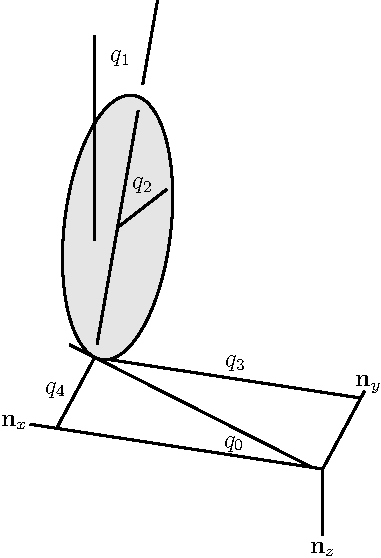
\includegraphics{rollingdisc.pdf}
%  \caption{Rolling disc configuration}
%  \label{fig:disc}
%\end{figure}
%
%The matrices which make up the linear equations were created using the method
%presented in Section \ref{sec:results}. It is important to note that the
%entries in these matrices must be evaluated at the point of linearization
%($\bm{q}^*, \bm{\dot{q}}^*, \bm{u}^*, \bm{\dot{u}}^*$), and that this point of
%linearization must satisfy the equations in Table \ref{table:assumptions}.
%There is no requirement that this point be an equilibrium point, which implies
%that in general both $\bm{\dot{q}}$ and $\bm{\dot{u}}$ may be non-zero. To
%reduce the complexity of the equations, we chose $q_0^* = q_2^* = 0$.  This
%means that the other quantities in the linearized equations (other $q$'s, the
%$\dot{q}$'s, the $u$'s, and the $\dot{u}$'s) need to be solved for with these 2
%quantities already set to 0.
%
%The independent state vector is:
%\begin{align}
%\begin{bmatrix}
%\delta \bm{q}_i \\
%\delta \bm{u}_i
%\end{bmatrix} =
%\begin{bmatrix}
%q_0 &
%q_1 &
%q_2 &
%q_3 &
%q_4 &
%u_0 &
%u_1 &
%u_2
%\end{bmatrix}^T
%\end{align}
%
%And the complete (independent and dependent) state vector is:
%\begin{align}
%\begin{bmatrix}
%\delta \bm{q} \\
%\delta \bm{u}
%\end{bmatrix} =
%\left[
%\begin{array}{cccccccccccc}
%q_0 &
%q_1 &
%q_2 &
%q_3 &
%q_4 &
%q_5 &
%u_0 &
%u_1 &
%u_2 &
%u_3 &
%u_4 &
%u_5
%\end{array}
%\right]^T
%\end{align}
%
%The coefficient matrices of the linearized equations (Equation
%\ref{eq:state_space_constrained}) are:
%\begin{equation}
%  \left[
%    \begin{array}{cc}
%      \tilde{M}_{qq} & \bm{0}_{n \times o} \\
%      \tilde{M}_{uqc} & \tilde{M}_{uuc} \\
%      \tilde{M}_{uqd} & \tilde{M}_{uud}
%    \end{array}
%    \right]=
%\left[\begin{smallmatrix}0 & 1 & 0 & 0 & 0 & 0 & 0 & 0 & 0 & 0 & 0 & 0\\s_{1} & 0 & 1 & 0 & 0 & 0 & 0 & 0 & 0 & 0 & 0 & 0\\c_{1} & 0 & 0 & 0 & 0 & 0 & 0 & 0 & 0 & 0 & 0 & 0\\0 & 0 & 0 & 1 & 0 & 0 & 0 & 0 & 0 & 0 & 0 & 0\\0 & 0 & 0 & 0 & c_{1} & s_{1} & 0 & 0 & 0 & 0 & 0 & 0\\0 & 0 & 0 & 0 & - s_{1} & c_{1} & 0 & 0 & 0 & 0 & 0 & 0\\0 & 0 & 0 & 0 & 0 & 0 & 0 & r & 0 & 1 & 0 & 0\\0 & 0 & - r u_{2} & 0 & 0 & 0 & - r & 0 & 0 & 0 & 1 & 0\\0 & 0 & r u_{1} & 0 & 0 & 0 & 0 & 0 & 0 & 0 & 0 & 1\\0 & 0 & 0 & 0 & 0 & 0 & - \frac{1}{4} m r^{2} & 0 & 0 & 0 & - m r & 0\\0 & 0 & 0 & 0 & 0 & 0 & 0 & - \frac{1}{2} m r^{2} & 0 & m r & 0 & 0\\0 & 0 & 0 & 0 & 0 & 0 & 0 & 0 & - \frac{1}{4} m r^{2} & 0 & 0 & 0\end{smallmatrix}\right]
%\end{equation}
%
%
%\begin{equation*}
%   \left[
%     \begin{array}{cc}
%       (\tilde{A}_{qq} + \tilde{A}_{qu} C_1 ) C_0 & \tilde{A}_{qu} C_2 \\
%       (\tilde{A}_{uqc} + \tilde{A}_{uuc} C_1 ) C_0 & \tilde{A}_{uuc} C_2\\
%       (\tilde{A}_{uqd} + \tilde{A}_{uud} C_1 ) C_0 & \tilde{A}_{uud} C_2
%     \end{array}
%   \right]=
%\end{equation*}
%\begin{equation}
%\left[\begin{smallmatrix}0 & 0 & c_{1} \dot{q}_{0} & 0 & 0 & 1 & 0 & 0\\0 & - c_{1} \dot{q}_{0} & 0 & 0 & 0 & 0 & 1 & 0\\0 & s_{1} \dot{q}_{0} & - \dot{q}_{1} & 0 & 0 & 0 & 0 & 1\\- \dot{q}_{4} & 0 & c_{1} \dot{q}_{5} - s_{1} \dot{q}_{4} & 0 & 0 & 0 & - r & 0\\c_{1} \dot{q}_{3} & - c_{1} \dot{q}_{5} + s_{1} \dot{q}_{4} & r u_{2} & 0 & 0 & r & 0 & 0\\- s_{1} \dot{q}_{3} & c_{1} \dot{q}_{4} + s_{1} \dot{q}_{5} & - r u_{1} - \dot{q}_{3} & 0 & 0 & 0 & 0 & 0\\0 & 0 & r u_{1} \dot{q}_{2} & 0 & 0 & 0 & 0 & 0\\0 & 0 & - r u_{0} \dot{q}_{2} & 0 & 0 & 0 & 0 & r \dot{q}_{2}\\0 & 0 & 0 & 0 & 0 & 0 & - r \dot{q}_{2} & 0\\0 & - c_{1} g m r & m r^{2} u_{0} u_{1} & 0 & 0 & - m r u_{5} & - \frac{5}{4} m r^{2} u_{2} & \frac{1}{4} m r \left(- r u_{1} + 4 u_{3}\right)\\0 & 0 & m r \left(r u_{1} + r u_{2} - u_{0} u_{4} + u_{1} u_{3} - \dot{u}_{5}\right) & 0 & 0 & m r^{2} u_{2} & - m r u_{5} & m r u_{4}\\0 & 0 & m r \left(- g s_{1} - u_{0} u_{5} + u_{2} u_{3} + \dot{u}_{4}\right) & 0 & 0 & \frac{1}{4} m r^{2} u_{1} & \frac{1}{4} m r^{2} u_{0} & 0\end{smallmatrix}\right]
%\end{equation}
%
%With this example, we have used our linearization procedure to find linear
%equations of motion which respect the system's constraints. Parametric
%stability analysis (eigenvalue analysis) can now be performed on these
%equations.  These computations were implemented symbolically with the open
%source symbolic manipulator SymPy \cite{SymPy2012}.
%
\section{Conclusions}
A procedure for forming linearized equations of motion for constrained
multi-body systems has been presented.  This procedure can be implemented
symbolically or numerically, and handles configuration, velocity, and
acceleration level constraints. 

%TODO: mention if it is compatible with other procedures.

The procedure has been implemented
symbolically in the \texttt{sympy.physics.mechanics} sub-module of the open
source symbolic manipulator SymPy\cite{SymPy2012}.

\begin{acknowledgements}
 This material is based upon work partially supported by the National Science
 Foundation under award 0928339 and three Google Summer of Code projects (2009,
 2011, 2012).  Jason Moore, Thomas Johnston, Evan Sperber, and Andrew Kickertz
 provided valuable feedback during discussions of multibody dynamics and
 control.
\end{acknowledgements}

\appendix
% Not sure which bibliography style we are supposed to use
%\bibliographystyle{spphys}       % APS-like style for physics
%\bibliographystyle{spbasic}      % basic style, author-year citations
\bibliography{references}   % name your BibTeX data base
\bibliographystyle{spmpsci}      % mathematics and physical sciences
\end{document}
